\documentclass[17pt]{beamer}

\usepackage{amsmath}
\usepackage{mathtools}
\usepackage{listings}
\usepackage{graphicx}

\lstset{
  basicstyle=\footnotesize\ttfamily,
  showstringspaces=false
}

\begin{document}

\title{How To Build Tile Server Using OpenStreetMap tools and data}
\author{Andrii Mishkovskyi}
\date{March 2011}

\maketitle

% \AtBeginSection[] % Do nothing for \section*
% {
%   \begin{frame}<beamer>
%     \frametitle{Outline}
%     \tableofcontents[currentsection]
%   \end{frame}
% }

\AtBeginSubsection[] % Do nothing for \subsection*
{
  \begin{frame}<beamer>
    \frametitle{Outline}
    \tableofcontents[currentsubsection]
  \end{frame}
}

\section*{Outline}

\begin{frame}
  \frametitle{Outline}
  \tableofcontents
\end{frame}

\section{Objectives and prerequisites}

\begin{frame}{What will you learn?}
  \begin{itemize}
  \item Cartography basics
  \item How to render maps with Mapnik
  \item How to build basic map service with Flask
  \end{itemize}
\end{frame}

\begin{frame}{First of all}
  \begin{itemize}
  \item Grab the CD or flash with all the data from me
  \item Use materials at content.mishkovskyi.net/pycon2011
  \item Or use handouts
  \end{itemize}
\end{frame}

\section{Introduction}

\subsection{Definitions}

\begin{frame}
  \frametitle{Terms}
  \begin{description}
  \item[Map] Graphic representation of the geographical setting
  \item[Cartography] Science and practice of making maps
  \item[GIS] A system that collects, analyzes, manages or processes in any other way data linked to location.
  \end{description}
\end{frame}

\begin{frame}
  \frametitle{Applications of GIS}
  \begin{itemize}
  \item Geography
  \item Cartography
  \item Navigation
  \item Search engines
  \item Remote sensing, land surveying, urban planning \ldots{}
  \end{itemize}
\end{frame}

\begin{frame}
  \frametitle{Characteristics of maps}
  \begin{itemize}
  \item<1-> Reduction \uncover<2->{\(\implies\) Scale}
  \item<3-> Transformation \uncover<4->{\(\implies\) Map projection}
  \item<5-> Abstractions \uncover<6->{\(\implies\) Symbolism}
  \end{itemize}
\end{frame}

\begin{frame}
  \frametitle{Classification of maps}
  \begin{itemize}
  \item By scale -- small-scale world, large-scale your neighborhood
  \item By function -- general reference, thematic, charts
  \item By subject matter -- cadastre, plans
  \end{itemize}
\end{frame}


\subsection{Map projections}

\begin{frame}
  \frametitle{Projection}
  Conversion of spherical information into 2d pane
\end{frame}

\begin{frame}
  \frametitle{Characteristics of projection}
  \begin{itemize}
  \item Linear distortion (scale factor)
  \item Area distortion
  \item Angle distortion
  \item Distance distortion
  \end{itemize}
\end{frame}

\begin{frame}
  \frametitle{Types of projections by surface}
  \begin{itemize}
  \item Conical
  \item Cylindrical
  \item Conformal
  \item
  \end{itemize}
\end{frame}

\begin{frame}
  \frametitle{Tissot indicatrix}
  \begin{block}{Representation of map distortions}
    \begin{center}
      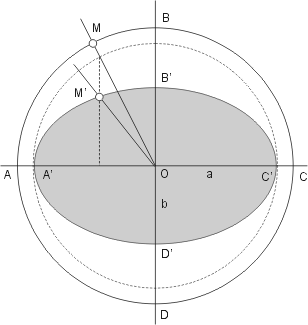
\includegraphics[scale=0.5]{pycon-2011-tutorial-files/indicatrix.png}
    \end{center}
  \end{block}
  \begin{block}{Distortions}
    \begin{description}
    \item[Linear] If $OA \neq OA'$ or $OB \neq OB'$
    \item[Angle]
    \item[Area] $OB' \times OA \neq OA \times OB'$
    \end{description}

  \end{block}
\end{frame}

\begin{frame}
  \frametitle{Mercator projection}
\only<2>{
  \begin{center}
    \begin{block}{Description}
      \begin{itemize}
      \item Conformal cylindrical projection
      \item No angle distortion
      \item Major area and linear distortion around poles
      \item Historically used for navigation
      \end{itemize}
    \end{block}
  \end{center}
}
\only<1>{
  \begin{block}{Tissot's indicatrix}
    \begin{center}
      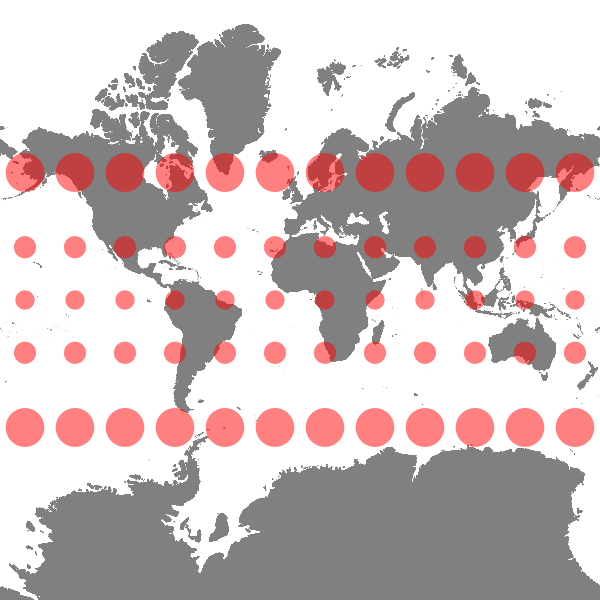
\includegraphics[scale=0.25]{pycon-2011-tutorial-files/merc-indicatrix.png}
    \end{center}
  \end{block}
}
\end{frame}

\begin{frame}
  \frametitle{Mollweide Projection}
\only<2>{
  \begin{block}{Description}
    \begin{itemize}
    \item Pseudocylindrical equal-area projection
    \item Serious linear and angle distortion
    \item Useful where area size is important (global distributions, visual
      area size comparison, etc)
    \end{itemize}
  \end{block}
}
\only<1>{
  \begin{block}{Tissot's indicatrix}
    \begin{center}
      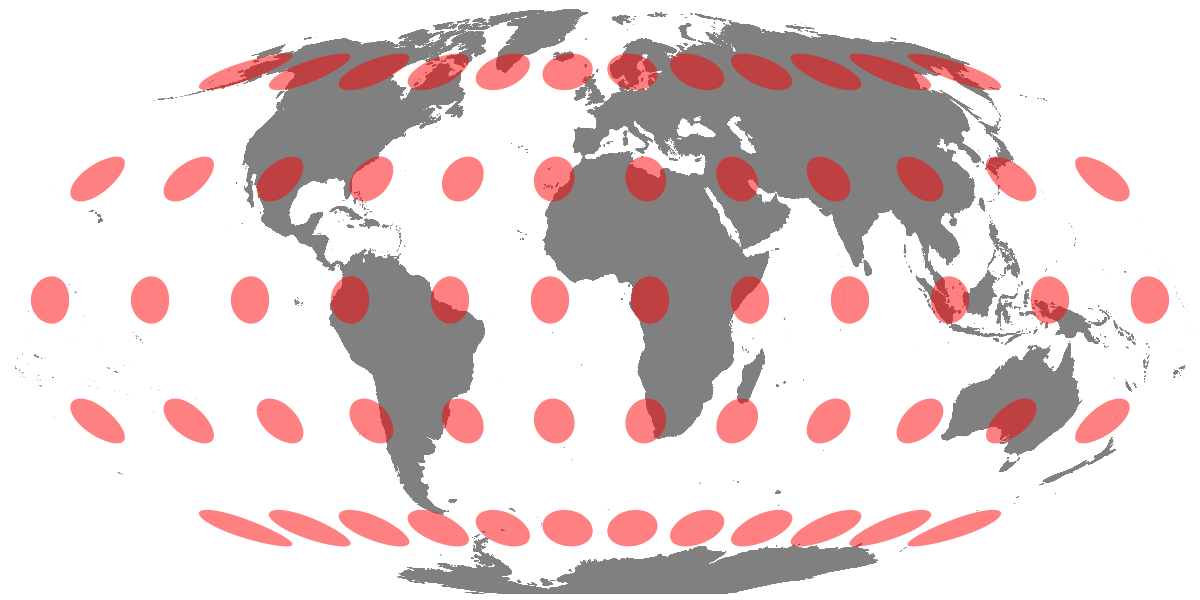
\includegraphics[scale=0.25]{pycon-2011-tutorial-files/moll-indicatrix.png}
    \end{center}
  \end{block}
}
\end{frame}

\subsection{Spatial data}

\begin{frame}
  \frametitle{Classes of data}
  \begin{itemize}
  \item Physical (Topographical -- elevations, terrain \& water objects)
  \item Cultural
  \item Human-made
  \end{itemize}
\end{frame}

\begin{frame}
  \frametitle{Sources of data}
  \begin{itemize}
  \item Mapping companies (TeleAtlas, Navteq, Ordnance Survey)
  \item Public sources (OpenStreetMap, Natural Earth)
  \item Government institutions (NASA, local government)
  \item Personal data (GPS tracks, social networks)
  \end{itemize}
\end{frame}

\begin{frame}
  \frametitle{Collecting data}
  \begin{itemize}
  \item Surveying
  \item GPS tracks
  \item Tracing aerial imagery
  \end{itemize}
\end{frame}

\begin{frame}
  \frametitle{Storing data}
  \begin{itemize}
  \item RDBMS (PostgreSQL + PostGIS, MySQL Spatial, Oracle Spatial, Spatialite)
  \item Non-relational databases (Neo4j, MongoDB, CouchDB)
  \item Flat files (WKB, WKT, GeoJSON, KML, GML)
  \end{itemize}
\end{frame}

\begin{frame}
  \frametitle{Simple Feature acess: SQL}
  \begin{itemize}
  \item Full set of querying functions
  \item Tons of useful features for on-the-fly projecting etc.
  \item Almost fully supported by PostGIS
  \end{itemize}
\end{frame}

\begin{frame}
  \frametitle{Other standards}
  \begin{itemize}
  \item Well-known text/binary
  \item Keyhole Markup Language
  \item Geography Markup Language
  \item Esri Shapefiles
  \end{itemize}
\end{frame}

\begin{frame}
  \frametitle{How OSM handles data}
  Special XML format used in
  \begin{itemize}
  \item Official API
  \item Official plant extracts
  \item Unofficial eXtended API (XAPI)
  \end{itemize}
\end{frame}

\begin{frame}[t]
  \frametitle{OSM data primitives}
  \begin{description}
  \item[Node] \only<1>{Stands for one geospatial point.}
  \item[Way] \only<2>{Collection of nodes. Can be used to represent
    such geometric features as lines (roads, borders, etc)
    and polygons (parks, buildings, etc.).}
  \item[Relation] \only<3>{Collection of other primitives (including
    relations themselves). Used for storing complex
    relationships between geospatial objects.}
  \end{description}
\end{frame}

\begin{frame}[fragile]
  \frametitle{How OSM XML looks like}
  \lstinputlisting[language=XML]{osm-xml-overview.xml}
\end{frame}

\begin{frame}
  \frametitle{Nodes}
  \lstinputlisting[language=XML]{osm-nodes-overview.xml}
\end{frame}

\begin{frame}
  \frametitle{Ways}
  \lstinputlisting[language=XML]{osm-ways-overview.xml}
\end{frame}

\begin{frame}
  \frametitle{Relations}
  \lstinputlisting[language=XML]{osm-relations-overview.xml}
\end{frame}

\begin{frame}
  \frametitle{Parsing OSM data}
  \begin{itemize}
  \item Osmosis
  \item osm2pgsql
  \item imposm
  \item tons of little scripts
  \end{itemize}
\end{frame}

\begin{frame}[t]
  \frametitle{osm2pgsql}
  \only<1>{Imports data to PostgreSQL with the following table setup}
  \begin{description}
  \item[planet\_osm\_point] \only<2>{Stores features which are represented with single symbol,
    such as bus stops, hotels (if mapped as points), ATMs, etc.}
  \item[planet\_osm\_line] \only<3>{Almost 90\% is take by different types of roads.}
  \item[planet\_osm\_polygon] \only<4>{Buildings, parks, etc.}
  \end{description}
\end{frame}

\begin{frame}
  \frametitle{Fetching data from PostgreSQL}
  \lstinputlisting[language=SQL]{simple-sql-query.sql}
\end{frame}

\begin{frame}
  \frametitle{Limiting search by bounding box}
  \lstinputlisting{sql-query-with-bbox.sql}[language=SQL]
\end{frame}

\begin{frame}
  \frametitle{More silly examples}
  \lstinputlisting{sql-examples.sql}[language=SQL]
\end{frame}

\section{Mapnik}

\begin{frame}
  \frametitle{What is Mapnik}
  Map rendering framework, written in \texttt{C++} with built-in \texttt{Python} bindings.
\end{frame}

\begin{frame}
  \frametitle{Mapnik concepts}
  \begin{description}
  \item[Symbolizer] \only<1>{Drawing rule of given geometric feature}
  \item[Rule] \only<2>{Collection of symbolizers for various data inputs.}
  \item[Style] \only<3>{Collection of rules. Exists mostly of convenience
    for defining layers.}
  \item[Datasource] \only<4>{Source of geospatial data.}
  \item[Layer] \only<5>{Link between datasource and styles}
  \item[Map] \only<6>{Abstraction over links between styles and layers}
  \end{description}
\end{frame}

\subsection{Hello World in Mapnik}

\begin{frame}
  \frametitle{Rendering map}
  \only<1>{
    \begin{center}
      \lstinputlisting{pycon-2011-tutorial-files/hw-import.py}
    \end{center}
  }
  \only<2>{
    \begin{center}
      \lstinputlisting{pycon-2011-tutorial-files/hw-rules.py}
    \end{center}
  }
  \only<3>{
    \begin{center}
      \lstinputlisting{pycon-2011-tutorial-files/hw-styles.py}
    \end{center}
  }
  \only<4>{
    \begin{center}
      \lstinputlisting{pycon-2011-tutorial-files/hw-layers.py}
    \end{center}
  }
  \only<5>{
    \begin{center}
      \lstinputlisting{pycon-2011-tutorial-files/hw-map.py}
    \end{center}
  }
  \only<6>{
    \begin{center}
      \lstinputlisting{pycon-2011-tutorial-files/hw-image.py}
    \end{center}
  }
\end{frame}

\begin{frame}
  \frametitle{Loading map file}
  \only<1>{
    \begin{center}
      \lstinputlisting{pycon-2011-tutorial-files/hw-xml-import.py}
    \end{center}
  }
  \only<2>{
    \begin{center}
      \lstinputlisting{pycon-2011-tutorial-files/hw-image.py}
    \end{center}
  }
\end{frame}

\begin{frame}
  \frametitle{Creating map file}
  \only<1>{
    \begin{center}
      \lstinputlisting{pycon-2011-tutorial-files/hw-map.xml}
    \end{center}
  }
  \only<2>{
    \begin{center}
      \lstinputlisting{pycon-2011-tutorial-files/hw-style.xml}
    \end{center}
  }
  \only<3>{
    \begin{center}
      \lstinputlisting{pycon-2011-tutorial-files/hw-layer.xml}
    \end{center}
  }
\end{frame}

% \subsection{Mapnik map files}

% \begin{frame}
%   \frametitle{Overview of map file in XML}

% \end{frame}

% \begin{frame}
%   \frametitle{Defining styles in XML}

% \end{frame}

% \begin{frame}
%   \frametitle{Defining rules in XML}

% \end{frame}

% \begin{frame}
%   \frametitle{Defining layers in XML}

% \end{frame}

% \subsection{Real world example}

% \begin{frame}
%   \frametitle{Fonts and fontsets}

% \end{frame}

% \begin{frame}
%   \frametitle{Including PostGIS datasources}

% \end{frame}

% \begin{frame}
%   \frametitle{Changing level of details aka zoom levels}

% \end{frame}

% \begin{frame}
%   \frametitle{Adding roads}

% \end{frame}


% \begin{frame}
%   \frametitle{Adding POIs}

% \end{frame}


\section{Imagery server}

\subsection{Simple map requests}

\begin{frame}[fragile]
  \frametitle{Hello world API}
  \begin{block}{\ttfamily{http://localhost:5000/map}}
    \only<1>{
      \lstinputlisting{pycon-2011-tutorial-files/ts-hw-import.py}
    }
    \only<2>{
      \lstinputlisting{pycon-2011-tutorial-files/ts-hw-handler.py}
    }
    \only<3>{
      \lstinputlisting{pycon-2011-tutorial-files/ts-hw-utils-render.py}
    }
  \end{block}
\end{frame}

\subsection{Tile API}


\begin{frame}[fragile]
  \frametitle{Tile API}
  \begin{block}{\ttfamily{http://localhost:5000/0/0/0.png}}
    \only<1>{
      \lstinputlisting{pycon-2011-tutorial-files/ts-hw-tile-import.py}
    }
    \only<2>{
      \lstinputlisting{pycon-2011-tutorial-files/ts-hw-tile.py}
    }
    \only<3>{
      \lstinputlisting{pycon-2011-tutorial-files/ts-hw-utils-parse_coords.py}
    }
    \only<4>{
      \lstinputlisting{pycon-2011-tutorial-files/ts-hw-utils-pixel2latlon.py}
    }
  \end{block}
\end{frame}

% \subsection{Additional APIs}



% \begin{frame}
%   \frametitle{Starting with Flask}

% \end{frame}

% \begin{frame}
%   \frametitle{Adding map rendering}

% \end{frame}

% \begin{frame}
%   \frametitle{Word about tiles}

% \end{frame}

% \begin{frame}
%   \frametitle{OSM tile scheme}

% \end{frame}

% \begin{frame}
%   \frametitle{Bing tile scheme}

% \end{frame}

% \begin{frame}
%   \frametitle{Adding basic staticmaps}

% \end{frame}

% \begin{frame}
%   \frametitle{Utility functions}

% \end{frame}


% Let's see our first example
% ...
% Looks scary, but do not fear, we'll go through every part of this nice and easy

% First of all, let's look at the line with the projection. It conforms to the
% previously discussed way of producing projection descriptions used by Proj.4

% TODO: actual descriptions prior to this

% Then, there's a simple Map creation mechanism. Map contains so called layers,
% which define the way the image layers are stacked and styles, which are named
% collections of rules, which describe the way geographical features are going
% to be represented

% Layers

% In classic cartography layers represent the actual physical layer. That is,
% layers correspond to the topographic view

% Styles

% Styles are set of rules

% Rules

% They define the way geographical features get rendered in the image, within
% the given scale.




% Mapnik
% Style file, layers and datasources
% Fonts
% Symbolizers

% To tile server

% WMS
% Tile API
% Different ways
% Google, Bing, Mapquest, Yahoo
% Building tile server from scratch
% Staticmaps

% Flask + Mapnik

% Changing styles on the fly
% Staticmaps
% Get tiles in bounding box


% http://msdn.microsoft.com/en-us/library/bb259689.aspx

\end{document}
